\documentclass[letter,12pt]{article}
\usepackage[paperheight=27.94cm,paperwidth=21.59cm,bindingoffset=0in,left=3cm,right=2.0cm, top=3.5cm,bottom=2.5cm, headheight=200pt, headsep=1.0\baselineskip]{geometry}
\usepackage{graphicx,lastpage}
\usepackage{upgreek}
\usepackage{censor}
\usepackage[spanish,es-tabla]{babel}
\usepackage{pdfpages}
\usepackage{tabularx}
\usepackage{graphicx}
\usepackage{adjustbox}
\usepackage{xcolor}
\usepackage{colortbl}
\usepackage{rotating}
\usepackage{multirow}
\usepackage[utf8]{inputenc}
\usepackage{float}

\renewcommand{\tablename}{Tabla}
\usepackage{fancyhdr}
\pagestyle{fancy}


%
\begin{document}
%
   \title{\Huge{Informe Laboratorio 1}}

   \author{\textbf{Sección 4} \\  \\Pablo Muñoz R \\ e-mail: pablo.munoz5@mail.udp.cl}
          
   \date{Agosto de 2026}

   \maketitle
   
   \tableofcontents
 
  \newpage
  

\section{Descripción}

\begin{enumerate}
    \item  Usted empieza a trabajar en una empresa tecnológica que se jacta de poseer sistemas que permiten identificar filtraciones de información a través de Deep Packet Inspection (DPI).
    A usted le han encomendado auditar si efectivamente estos sistemas son capaces de detectar las filtraciones a través de tráfico de red. Debido a que el programa ping es ampliamente utilizado desde dentro y hacia fuera de la empresa, su tarea será crear un software que permita replicar tráfico generado por el programa ping con su configuración por defecto, pero con fragmentos de información confidencial. Recuerde que al comparar tráfico real con el generado no debe gatillar alarmas.
    De todas formas, deberá hacer una prueba de concepto, en la cual se demuestre que al conocer el algoritmo, será fácil determinar el mensaje en claro.
    Para los pasos 1,2,3 indicar el texto entregado a ChatGPT y validar si el código resultante cumple con lo requerido.


\end{enumerate}


\section{Actividades}


\subsection{Algoritmo de cifrado}

\begin{enumerate}
\item Generar un programa, en python3 utilizando chatGPT, que permita cifrar texto utilizando el algoritmo Cesar. Como parámetros de su programa deberá ingresar el string a cifrar y luego el corrimiento.
\begin{figure}[H]
        \centering
        \includegraphics[width=15cm]{actividades/A1.png}
        \label{fig:a1}
\end{figure}


\end{enumerate}

\subsection{Modo stealth}

\begin{enumerate}
    \item Generar un programa, en python3 utilizando ChatGPT, que permita enviar los caracteres del string (el del paso 1) en varios paquetes ICMP request (un caracter por paquete en el campo data de ICMP) para de esta forma no gatillar sospechas sobre la filtración de datos.
Deberá mostrar los campos de un ping real previo y posterior al suyo y demostrar que su tráfico consideró todos los aspectos para pasar desapercibido.
    \begin{figure}[H]
        \centering
        \includegraphics[width=15cm]{actividades/A2.1.png}
        \label{fig:a2-1}
    \end{figure}
    El último carácter del mensaje se transmite como una b.
    \begin{figure}[H]
            \centering
            \includegraphics[width=15cm]{actividades/A2.2.png}
            \label{fig:a2-2}
        \end{figure}
\end{enumerate}

\subsection{MitM}
\begin{enumerate}
    \item Generar un programa, en python3 utilizando ChatGPT, que permita obtener el mensaje transmitido en el paso2. Como no se sabe cual es el corrimiento utilizado, genere todas las combinaciones posibles e imprímalas, indicando en verde la opción más probable de ser el mensaje en claro.
    \begin{figure}[H]
        \centering
        \includegraphics[width=12cm]{actividades/A3.png}
        \label{fig:a3}
    \end{figure}
    Finalmente, deberá indicar 4 issues que haya tenido al lidiar con ChatGPT, netamente para reflejar cuál fue su experiencia al trabajar con esta tecnología.

\end{enumerate}

\section{Desarrollo de Actividades}

\subsection{Actividad 1}
Cifrado cesar: Se implementó ocupando DeepSeek un programa en python dedicado a aplicar cifrado cesar a palabras o frases completas. El algoritmo recorre cada carácter del texto, aplica el desplazamiento a las letras del alfabeto inglés (a-z, A-Z) y mantiene sin cambios los caracteres no alfabéticos para preservar la estructura del mensaje. 
\begin{figure}[H]
    \centering
    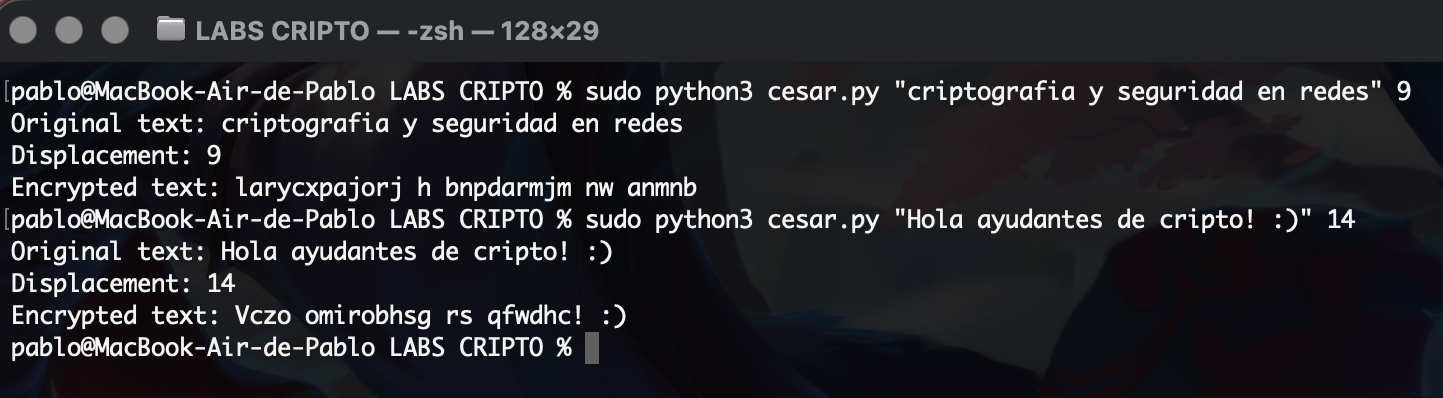
\includegraphics[width=0.9\linewidth]{cesar.terminal.png}
    \caption{Programa cesar.py corriendo en terminal}
    \label{fig:cesar}
\end{figure}


En la Figura \ref{fig:cesar} se observa el correcto funcionamiento del programa. Al cifrar \textit{``criptografia y seguridad en redes''} con desplazamiento 9, se obtiene \textit{``larycxpajorj h bnpdarmjm nw anmnb''}. La prueba con desplazamiento 14 sobre el texto \textit{''Hola ayudantes de cripto! :)''} confirma que el algoritmo funciona para distintos desplazamientos. Se recomienda consultar los anexos para observar el código en mayor profundidad.

\subsubsection*{Ingreso de argumentos por terminal}

El script \texttt{cesar.py} recibe dos argumentos por línea de comandos: el texto a cifrar y el corrimiento. Esto se evidencia en la Figura~\ref{fig:cesar}, donde se ejecuta:

\begin{verbatim}
sudo python3 cesar.py "criptografia y seguridad en redes" 9
\end{verbatim}

\subsection{Actividad 2}

\subsubsection{Modo stealth}

Para esta actividad se solicitó a DeepSeek la generación de un programa en Python3
(\texttt{pingv4.py}) capaz de transmitir, carácter por carácter, el mensaje cifrado
obtenido en la Actividad 1, utilizando paquetes ICMP
Echo Request (tipo 8) que replican en todos sus campos el comportamiento de un ping
real generado por el sistema operativo. El objetivo es evitar que un sistema de
inspección profunda de paquetes (DPI) distinga esta fuga de información del tráfico
ICMP legítimo.

\subsubsection*{Ingreso de argumentos por terminal}

El programa recibe como parámetros el texto a transmitir y, opcionalmente, la
dirección IP de destino. Si no se especifica una IP, se utiliza por defecto
\texttt{8.8.8.8}; si se indica \texttt{127.0.0.1}, el script activa explícitamente
el modo \emph{loopback}, lo que permite realizar pruebas de concepto sin generar
tráfico hacia el exterior de la red.

\begin{verbatim}
sudo python3 pingv4.py "larycxpajorj h bnpdarmjm nw anmnb" 127.0.0.1
\end{verbatim}

\begin{figure}[H]
    \centering
    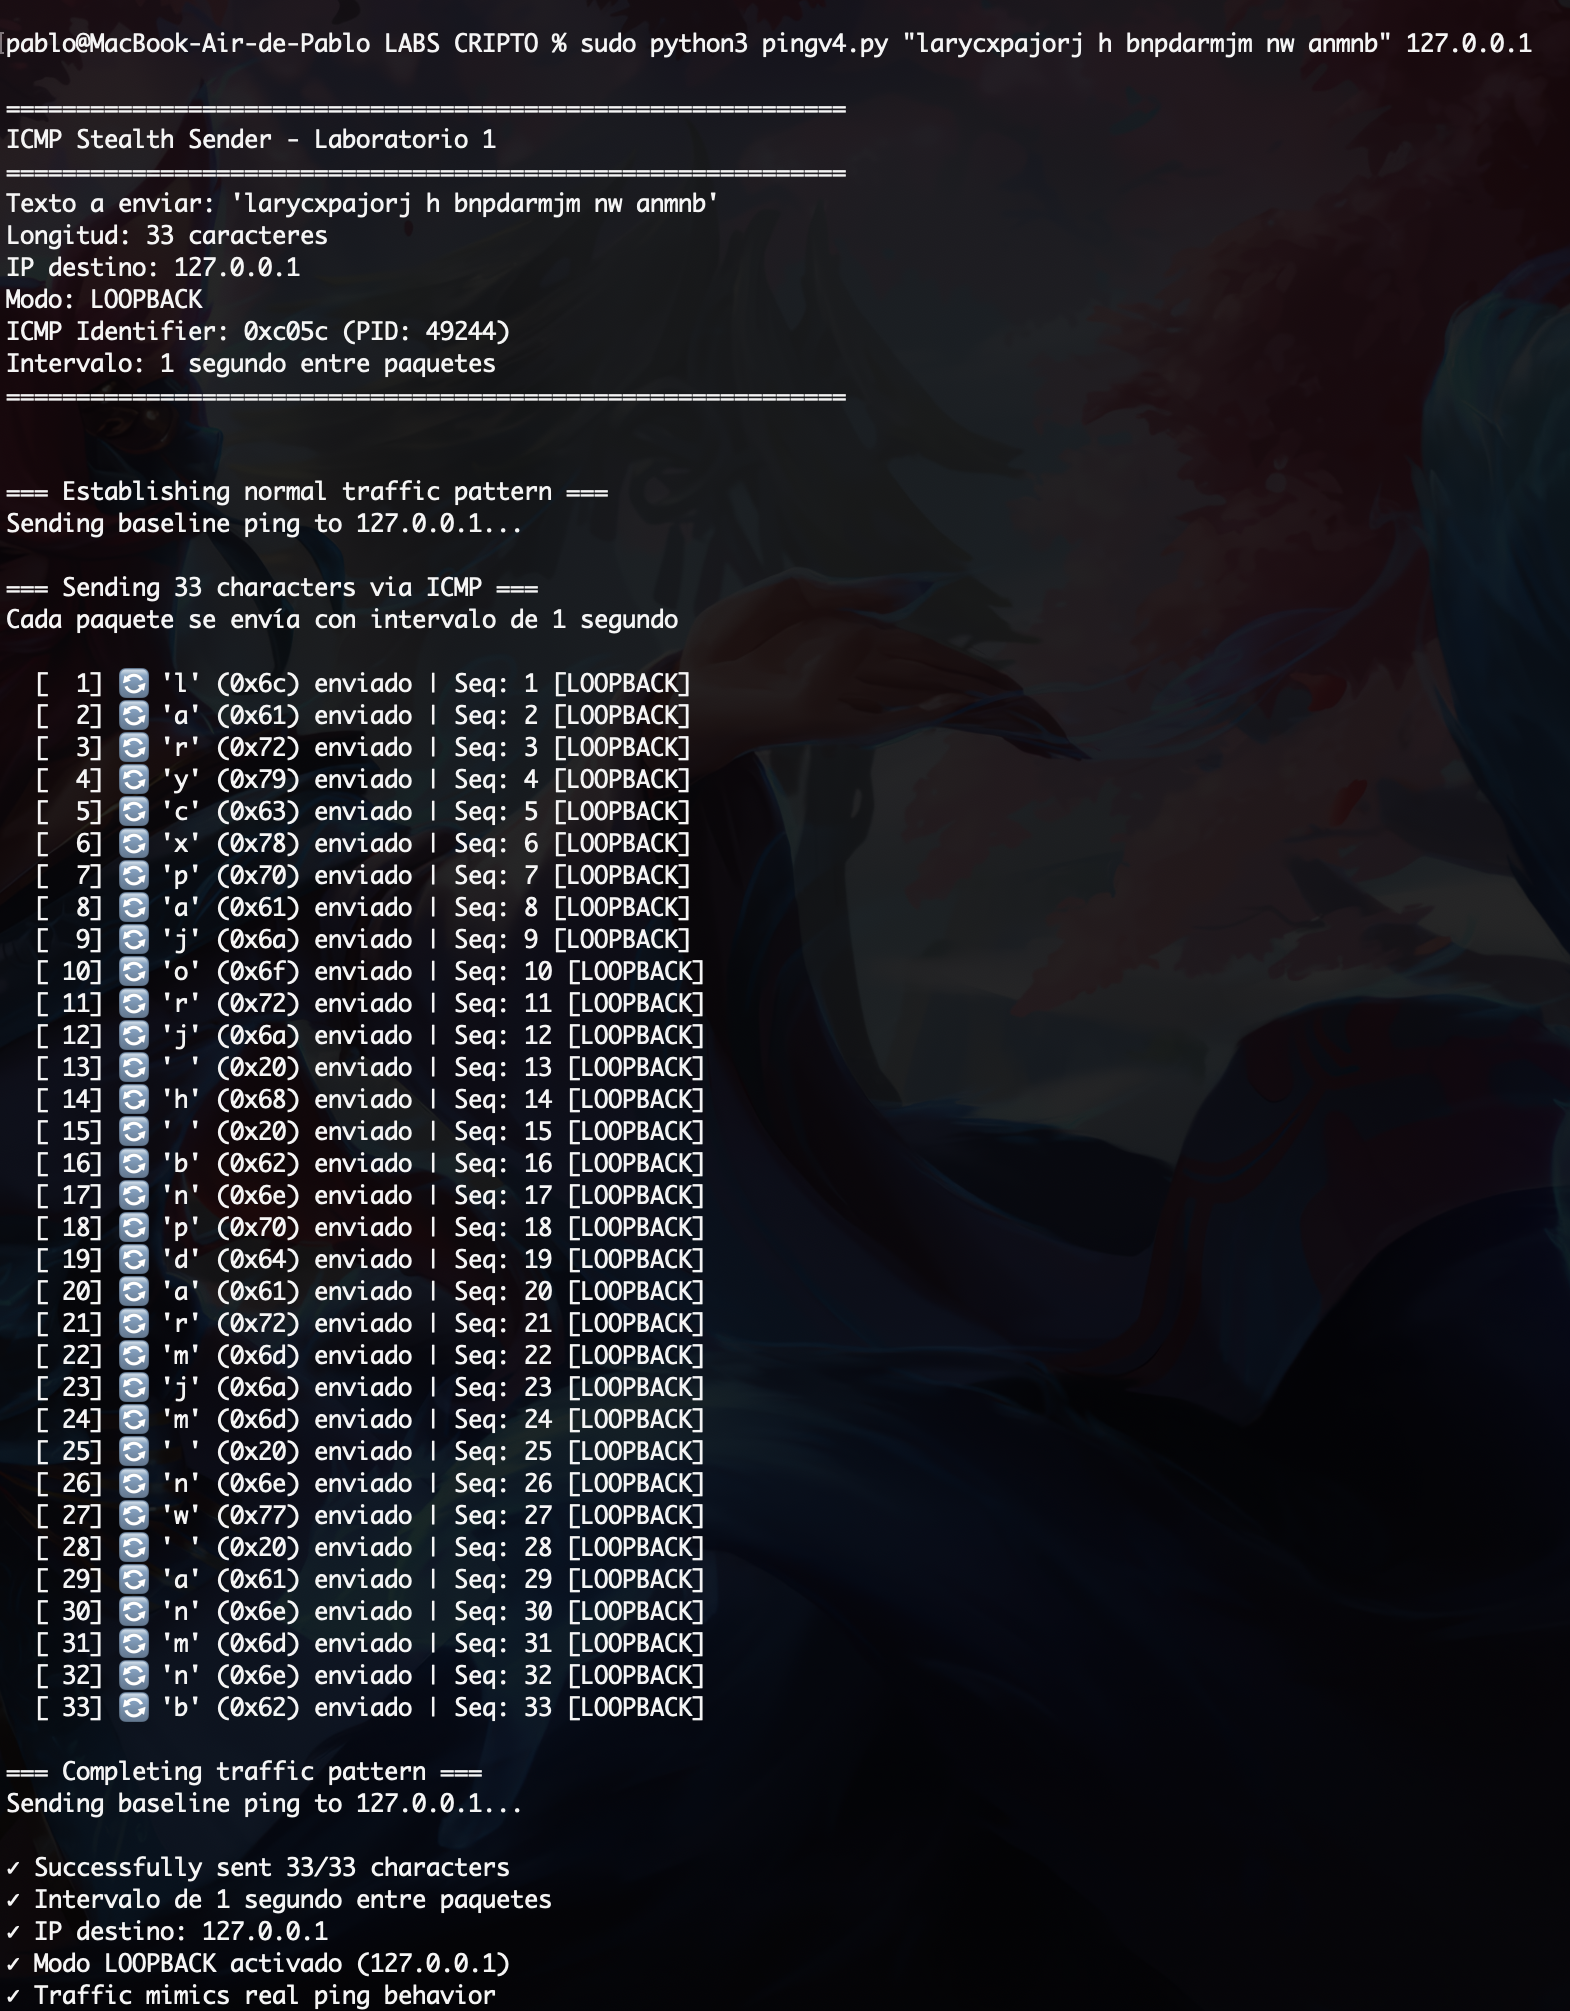
\includegraphics[width=0.8\textwidth]{LoopBACK_terminal.png}
    \caption{Ejecución de \texttt{pingv4.py} en modo loopback, mostrando el envío
    secuencial de cada carácter del mensaje cifrado.}
    \label{fig:stealth-terminal}
\end{figure}

\subsubsection*{Tráfico hacia IP de loopback}

Al ejecutar el script contra \texttt{127.0.0.1}, el tráfico ICMP generado pudo
capturarse localmente mediante Wireshark, lo que permitió verificar de forma directa
la estructura de cada paquete antes de ser enviado a un destino externo.

\begin{figure}[H]
    \centering
    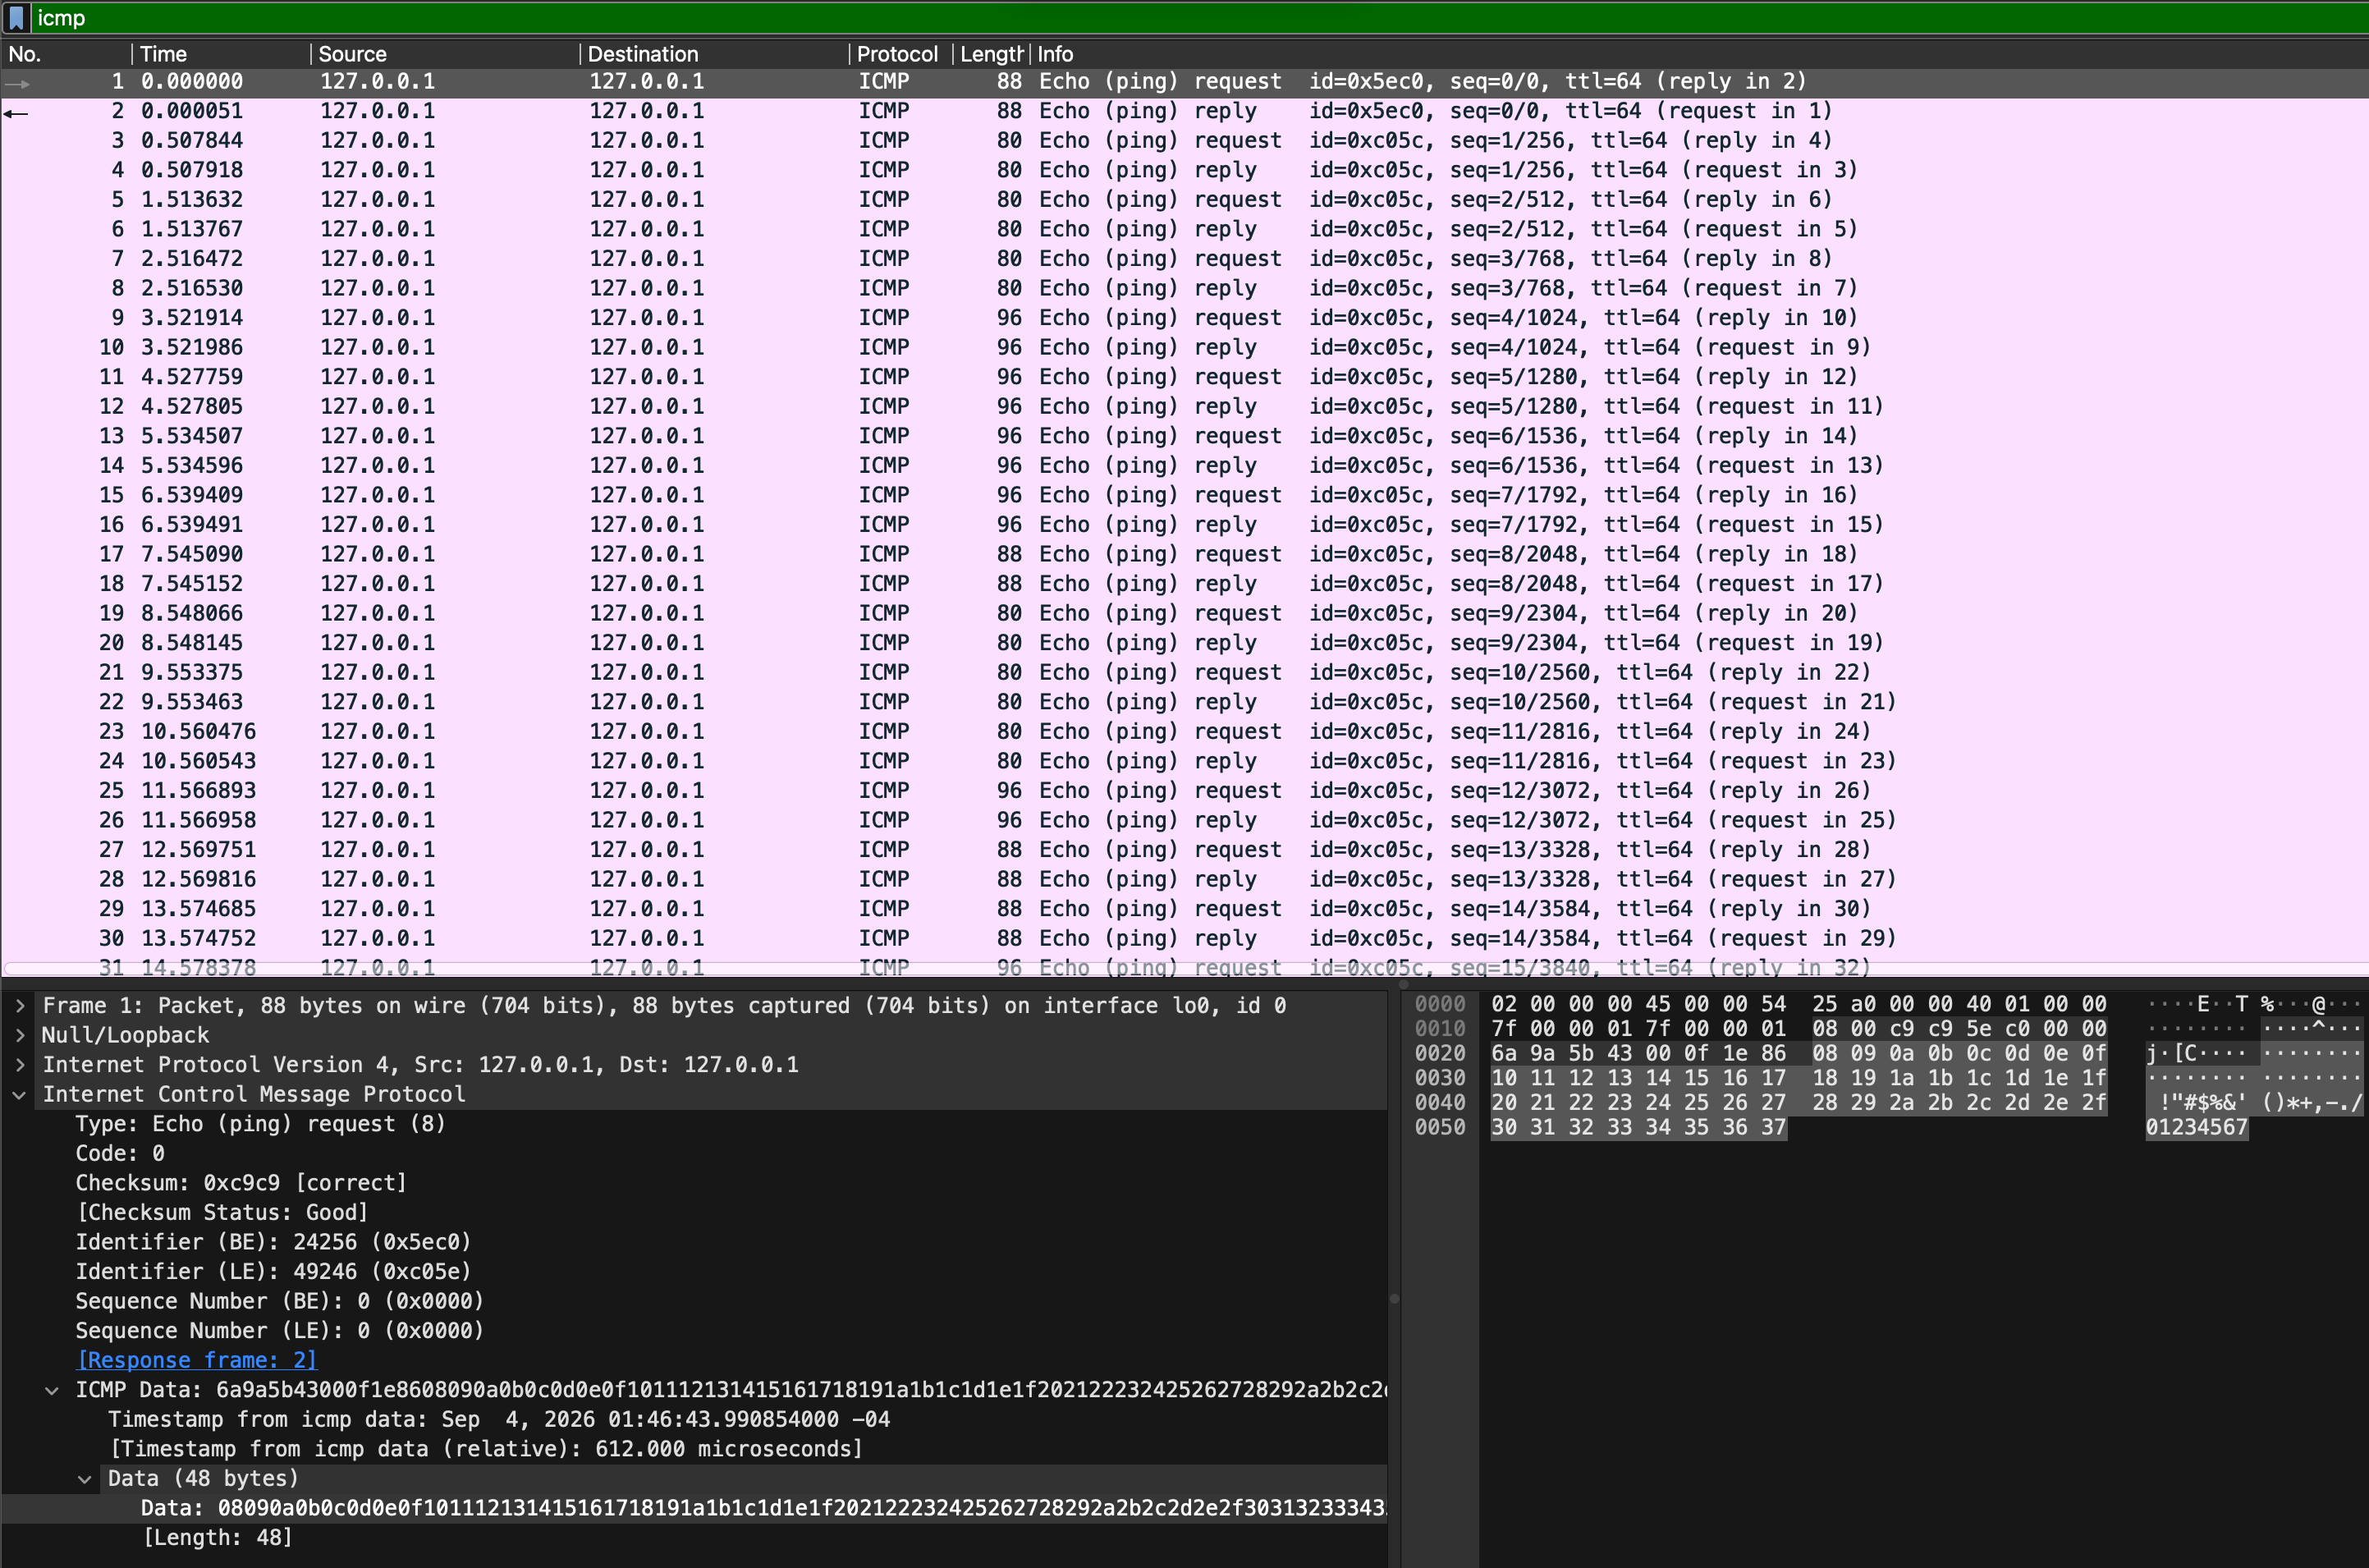
\includegraphics[width=1\textwidth]{wireshark_LB.png}
    \caption{Captura en Wireshark del tráfico ICMP dirigido a \texttt{127.0.0.1}.}
    \label{fig:stealth-loopback}
\end{figure}

\subsubsection*{Inyección del cifrado en el tráfico}

Cada paquete ICMP transporta, en su campo \emph{Data}, un único carácter del texto
cifrado con César obtenido en la Actividad 1. De esta forma, el mensaje completo
queda distribuido a lo largo de una secuencia de paquetes en apariencia normales,
en lugar de concentrarse en un solo paquete que resultaría sospechoso ante un
análisis de contenido.

\begin{figure}[H]
    \centering
    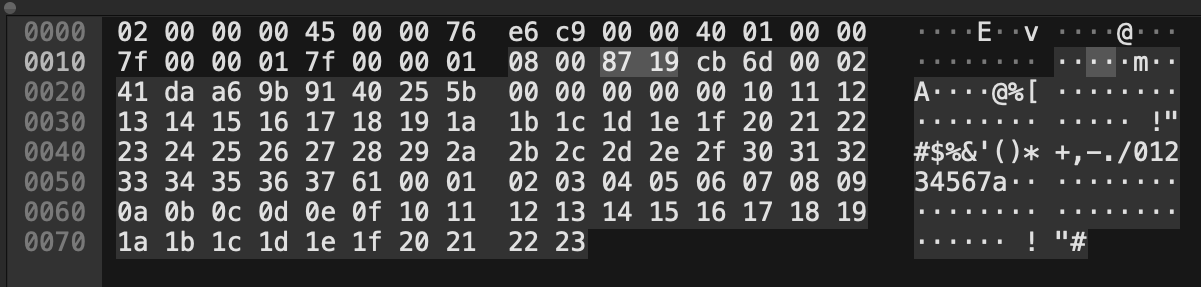
\includegraphics[width=1\textwidth]{WS_LBs.png}
    \caption{Payload ICMP mostrando el carácter inyectado \texttt{0x61} ('a') al final del patrón \texttt{0x10-0x37}.}
    \label{fig:stealth-payload}
\end{figure}

En la Figura~\ref{fig:stealth-payload} se observa el payload del paquete ICMP capturado en modo loopback. La estructura del payload es la siguiente: primero se aprecian los 8 bytes correspondientes al timestamp (bytes \texttt{41 da a6 9b 91 40 25 5b}), seguidos de los 5 bytes en \texttt{0x00} requeridos por el estándar del ping real. A continuación, se visualiza el patrón completo desde \texttt{0x10} hasta \texttt{0x37} (bytes \texttt{10 11 12 ... 35 36 37}). Finalmente, en la posición 53 del payload se encuentra el byte \texttt{0x61}, que corresponde al carácter \textit{`a`} del mensaje cifrado inyectado. El resto de los bytes corresponden al padding, utilizado para ajustar el tamaño del paquete al estándar del ping real.

\subsubsection*{Intervalo entre paquetes}

El script introduce una espera de
exactamente un segundo entre el envío de cada carácter, replicando el
comportamiento por defecto del comando \texttt{ping} y evitando ráfagas de tráfico
que pudieran llamar la atención de un sistema de monitoreo.

\subsubsection*{Coherencia de timestamp, IP identification y seq number}

Para que el tráfico generado sea indistinguible del tráfico real, el programa
mantiene coherencia en los siguientes campos:

\begin{itemize}
    \item \textbf{Timestamp ICMP}: cada paquete conserva un timestamp acorde al
    momento real de envío, igual que lo haría el comando \texttt{ping} nativo.
    \item \textbf{IP Identification}: el campo \texttt{IP ID} se incrementa de
    forma consistente entre paquetes, replicando el patrón que genera el sistema
    operativo al enviar pings sucesivos.
    \item \textbf{Sequence number (ICMP seq)}: se incrementa en cada paquete
    siguiendo el mismo orden que el índice del carácter transmitido, tal como lo
    haría una sesión real de ping.
    \item \textbf{ICMP identifier}: se fija un identificador único (derivado del
    PID del proceso) y se mantiene constante durante toda la sesión, replicando el
    comportamiento estándar de \texttt{ping}.
\end{itemize}



\begin{figure}[H]
    \centering
    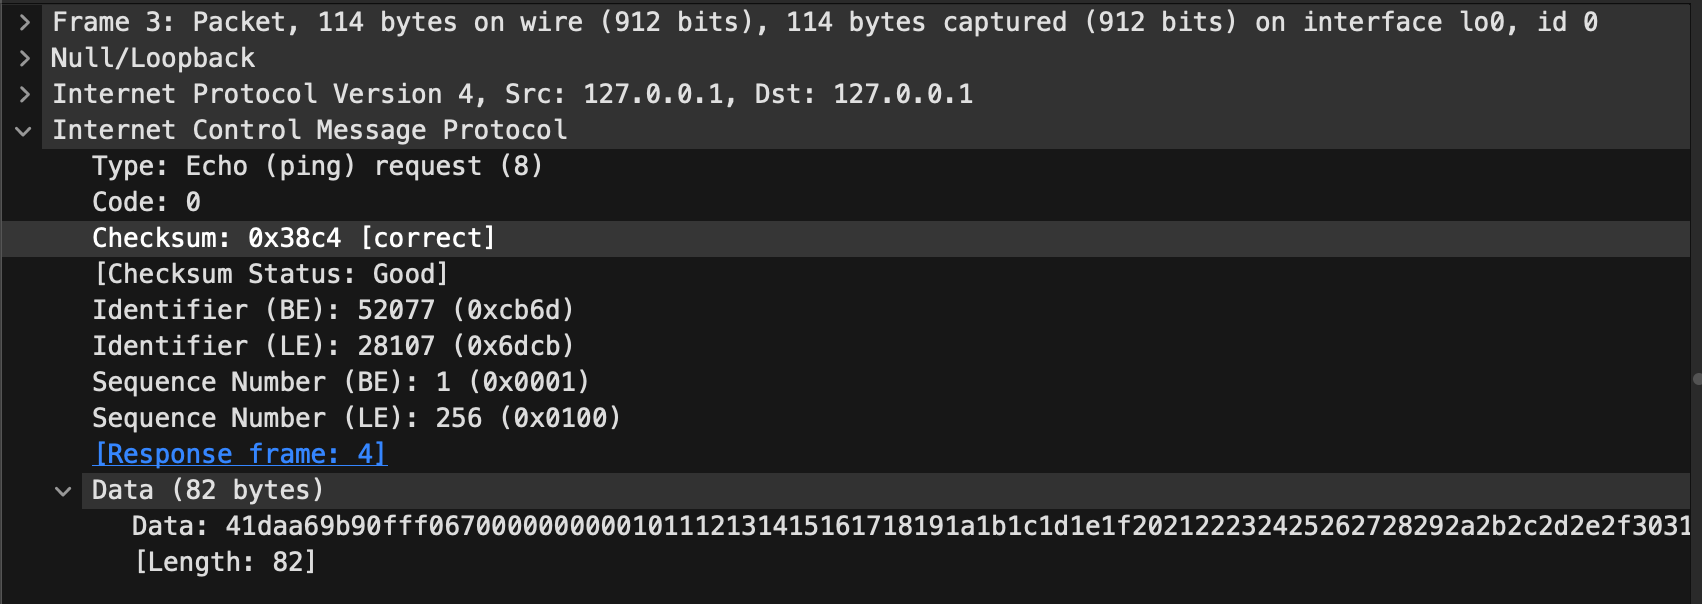
\includegraphics[width=0.9\textwidth]{F3.png}
    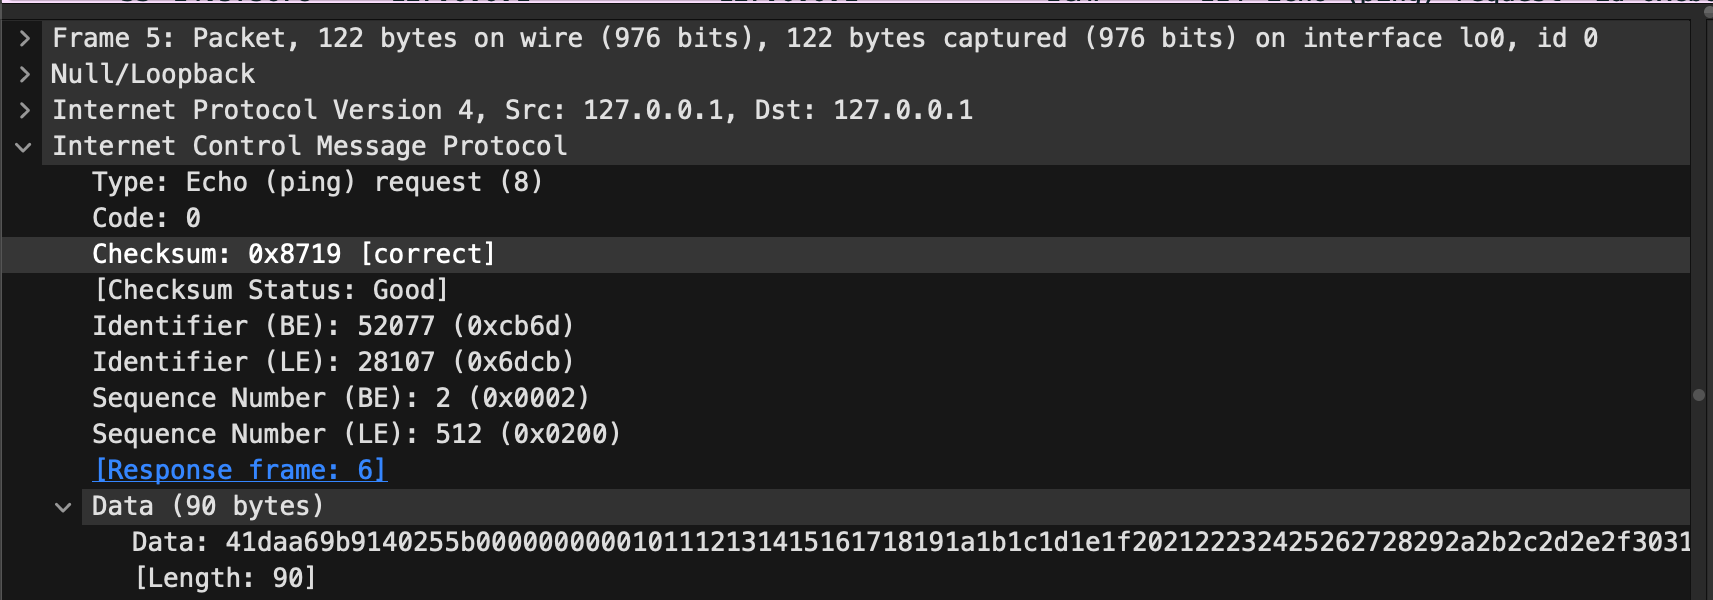
\includegraphics[width=0.9\textwidth]{F5.png}
    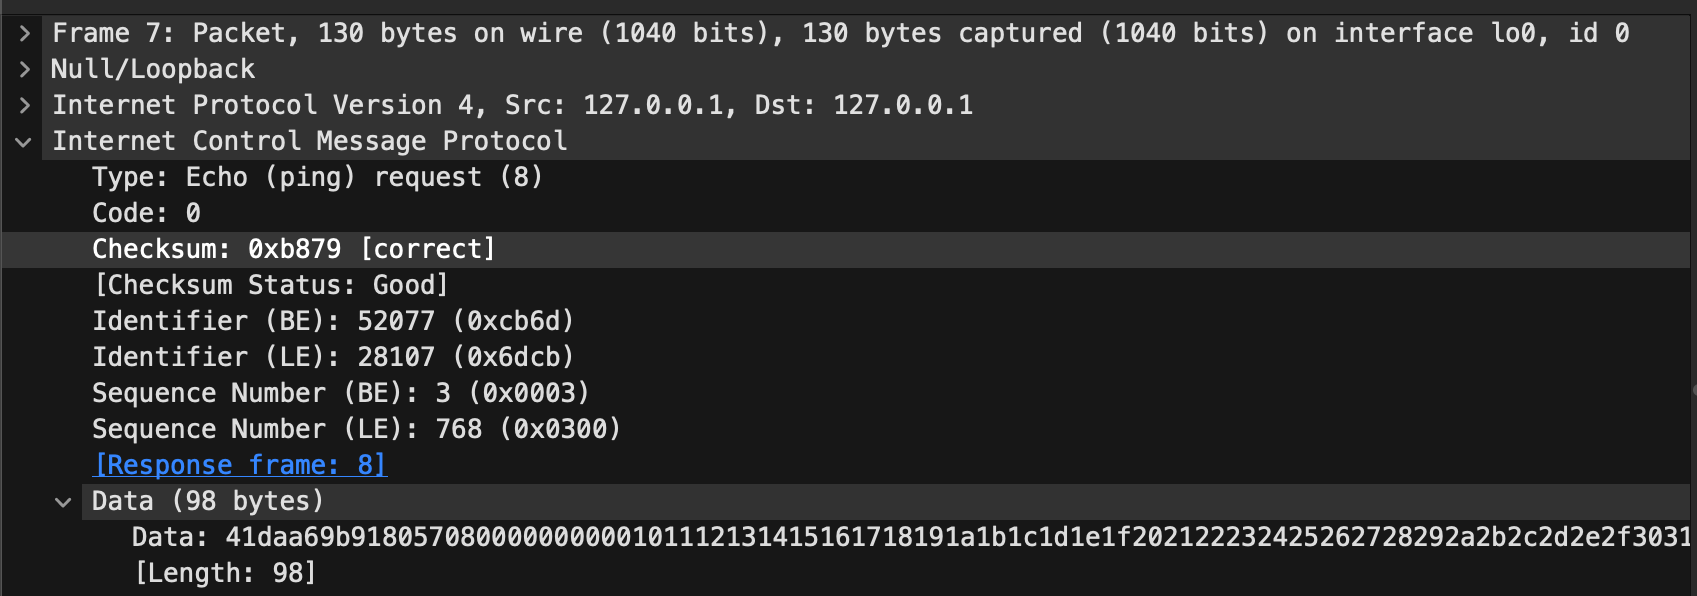
\includegraphics[width=0.9\textwidth]{F7.png}
    \caption{Muestra de 3 Frames correspondientes a el texto injectado en el tráfico}
    \label{fig:coherencia-campos}
\end{figure}

De la Figura~\ref{fig:coherencia-campos} se observa que los frames mantienen el mismo \textit{ICMP identifier} (\texttt{0xcb6d}) y el \textit{Sequence Number} incrementa de uno en uno (\texttt{0x0001}, \texttt{0x0002}, \texttt{0x0003}), replicando el comportamiento de un ping real. Además de tener cada checksum correcto.

\begin{figure}[H]
    \centering
    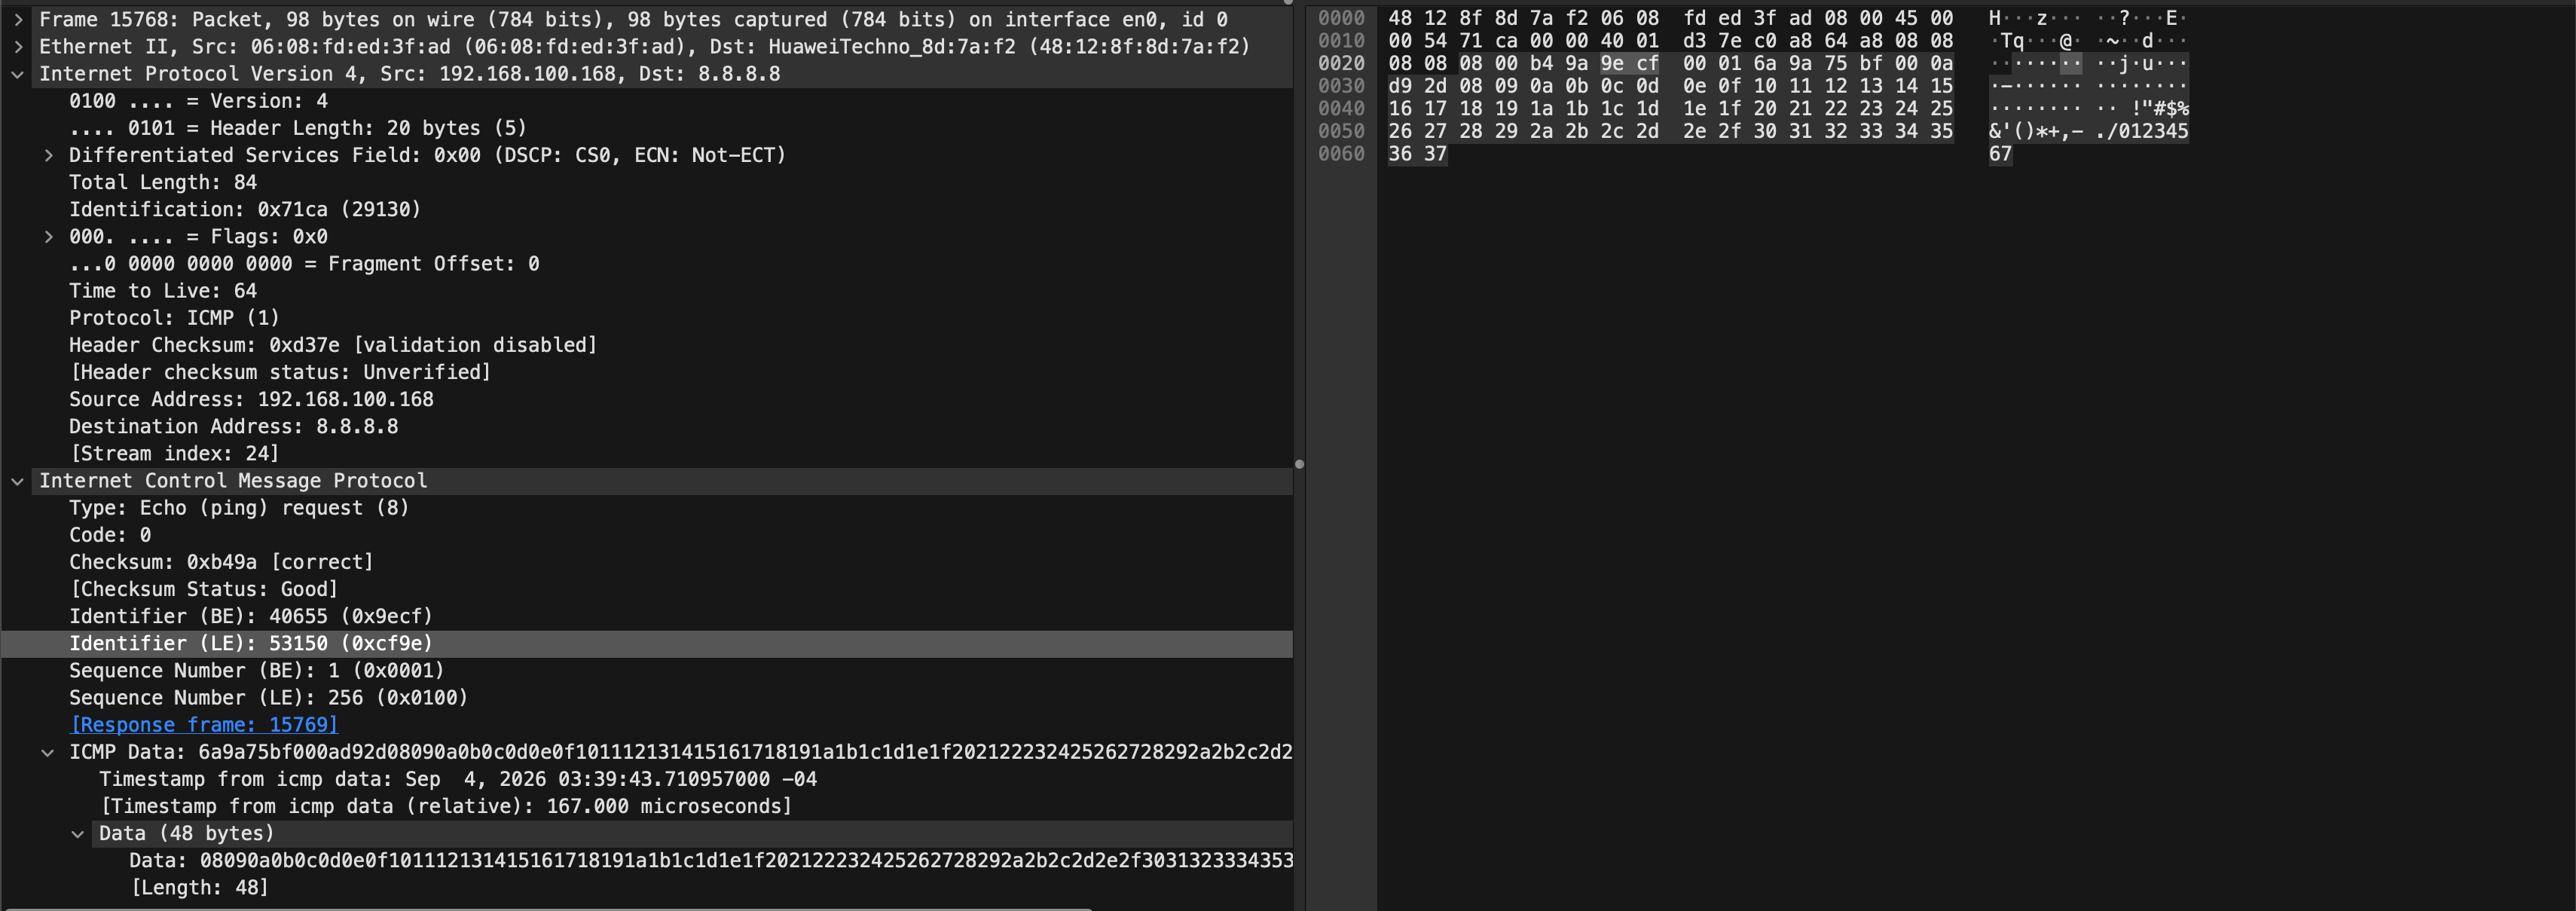
\includegraphics[width=1\textwidth]{real.png}
    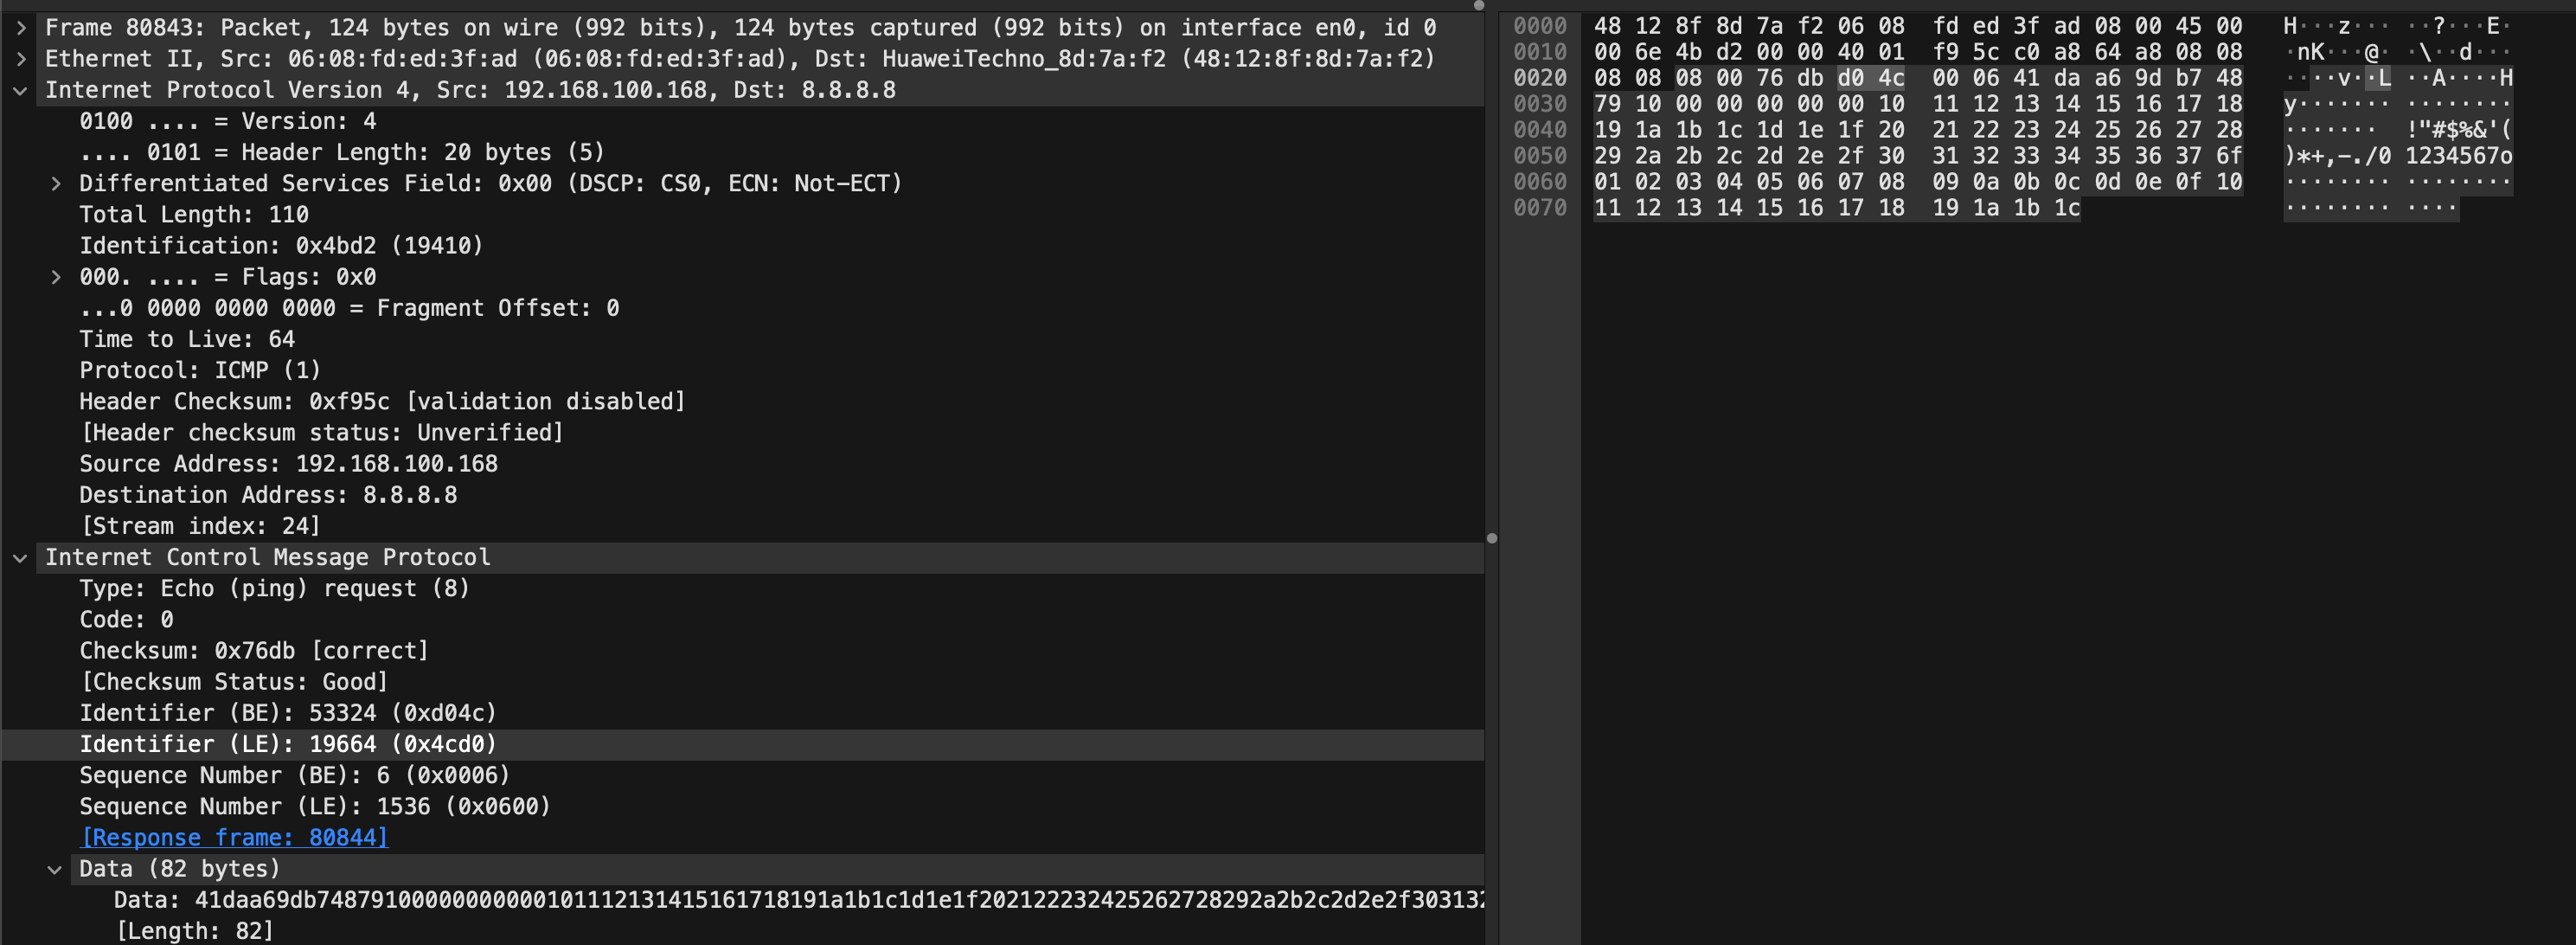
\includegraphics[width=1\textwidth]{script.png}

    \caption{Comparación de los campos ICMP (timestamp, ID, seq, identifier) entre
    un ping real(Arriba) y el generado por el script(Abajo).}
    \label{fig:comparacion}
\end{figure}

Ambos paquetes presentan las siguientes características comunes:
\begin{itemize}
    \item \textbf{Type:} 8 (Echo Request) en ambos casos.
    \item \textbf{Code:} 0 en ambos casos.
    \item \textbf{Checksum:} Correcto en ambos (\texttt{[Checksum Status: Good]}).
    \item \textbf{Identifier:} Constante durante cada ejecución (PID del proceso).
    \item \textbf{Sequence Number:} Incrementa secuencialmente.
    \item \textbf{Timestamp:} Presente en ambos payloads.
    \item \textbf{TTL:} 64 en ambos casos.
\end{itemize}

La comparación evidencia que el tráfico generado por \texttt{pingv4.py} es funcionalmente idéntico al de un ping real, manteniendo todos los campos ICMP coherentes y un checksum válido, lo que permite su uso como método de filtración sin levantar sospechas ante sistemas DPI.



\subsubsection*{Checksum coherente}

El checksum ICMP se recalcula para cada paquete en función del header y el payload
efectivamente enviados, siguiendo el mismo algoritmo estándar utilizado por el
protocolo ICMP. Esto garantiza que, al ser inspeccionado por cualquier herramienta
de análisis de tráfico, el paquete resulte válido y no genere alertas de
integridad.

Como evidencia adicional, se muestran los campos de un ping real inmediatamente
anterior y posterior a la secuencia de paquetes generados por el script,
confirmando que ambos tráficos resultan indistinguibles a nivel de estructura.


\subsection{Actividad 3}

Para esta actividad se implementó el script \texttt{readv2.py}, que permite capturar el tráfico ICMP generado por \texttt{pingv4.py}, extraer el mensaje cifrado del payload de los paquetes y recuperar el texto original mediante fuerza bruta del cifrado César.

El script soporta dos modos de operación:
\begin{itemize}
    \item \textbf{Lectura de PCAP}: Analiza un archivo \texttt{.pcap} capturado previamente con Wireshark o tcpdump.
    \item \textbf{Captura en vivo}: Escucha el tráfico ICMP en tiempo real utilizando Scapy.
\end{itemize}

Una vez obtenido el mensaje cifrado, el programa prueba las 26 combinaciones posibles del cifrado César y calcula la probabilidad de que cada una corresponda a texto en lenguaje natural. Para ello, utiliza:
\begin{itemize}
    \item \textbf{Análisis de frecuencia}: Compara la distribución de letras con tablas de frecuencia del español.
    \item \textbf{Diccionario}: Busca palabras comunes en español dentro del texto.
    \item \textbf{Estructura}: Evalúa la presencia de espacios y proporción de vocales.
\end{itemize}

La opción con mayor puntuación se muestra en \textcolor{green}{verde}, indicando el mensaje en claro y el corrimiento utilizado.

\subsubsection*{Ejemplo de ejecución}

En la Figura~\ref{fig:mitm-ejecucion} se muestra la ejecución de \texttt{readv2.py} sobre un archivo PCAP que contiene el tráfico generado por \texttt{pingv4.py}. El script reconstruye el mensaje cifrado \textit{``larycxojxrji h bnovjajrji nw anmcb''} y prueba las 26 combinaciones, identificando correctamente el mensaje original \textit{``criptografia y seguridad en redes''} con corrimiento 9.

\begin{figure}[H]
    \centering
    \begin{minipage}{0.48\textwidth}
        \centering
        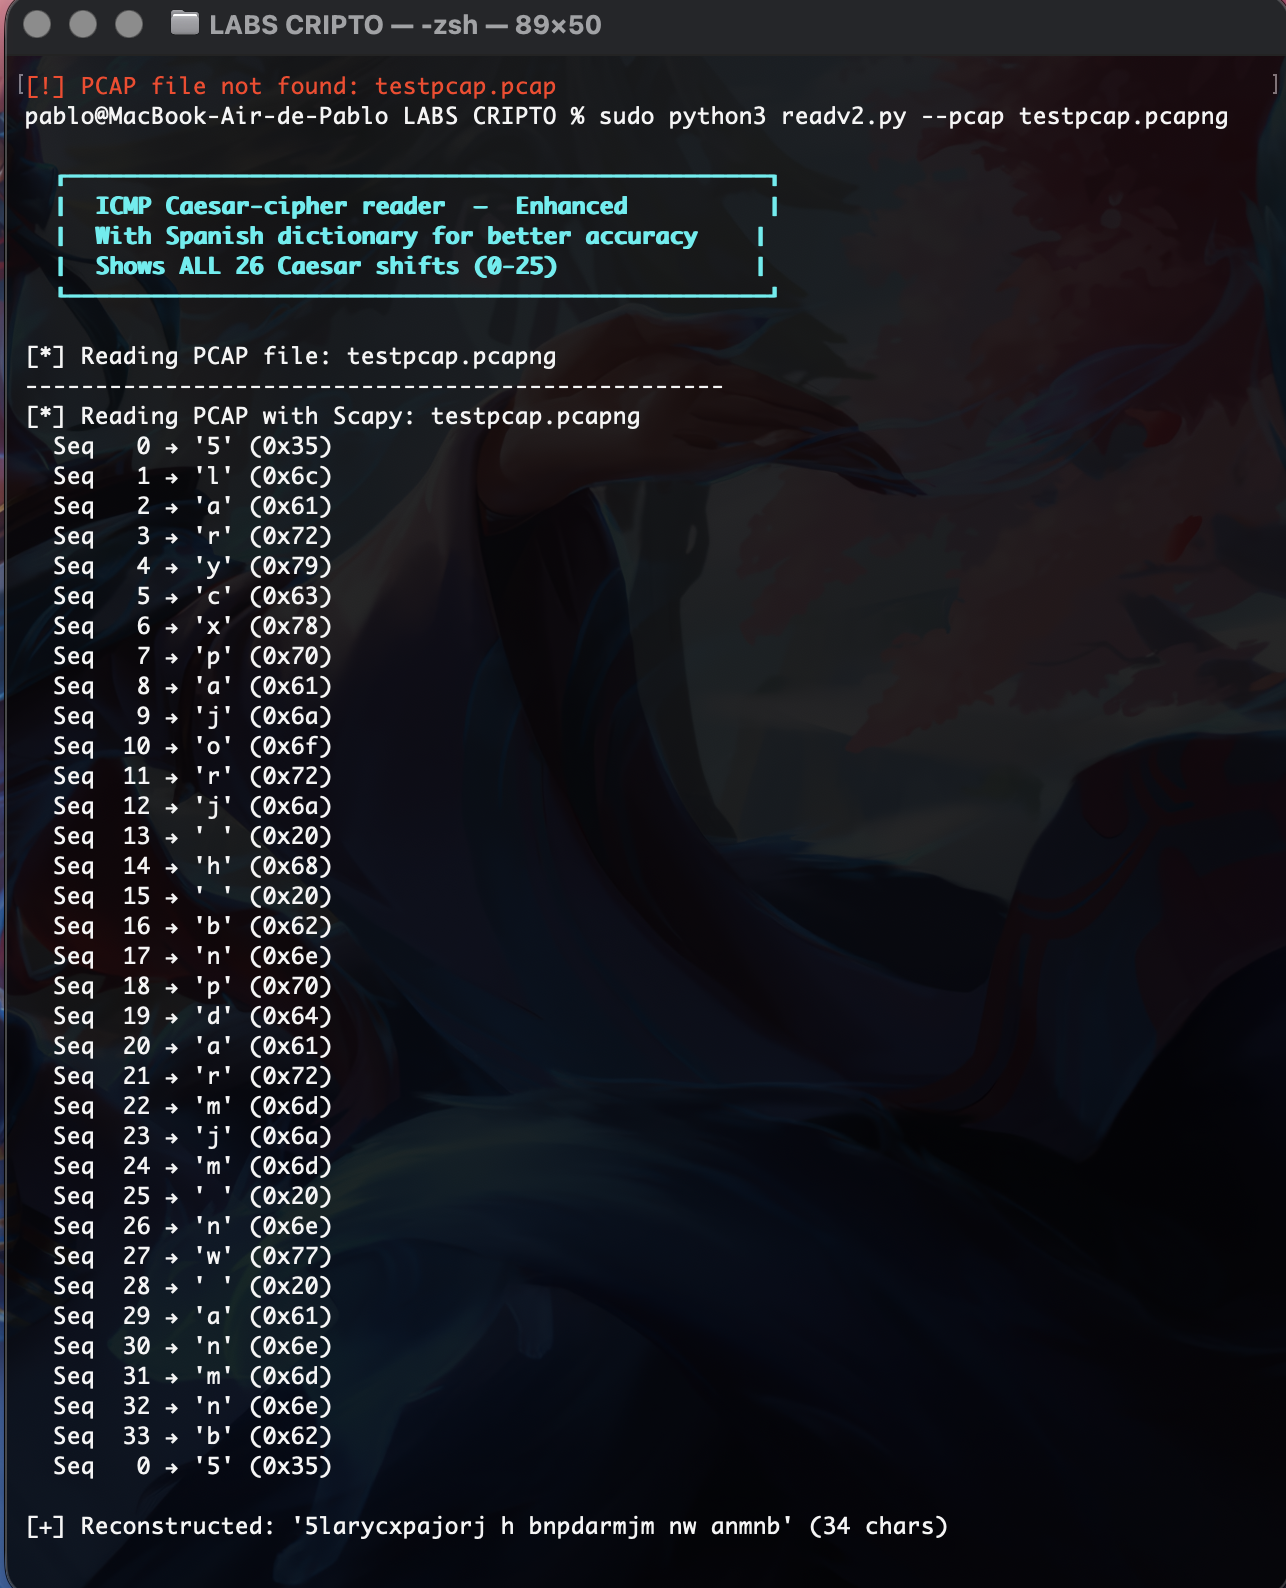
\includegraphics[width=\textwidth]{pcap1.png}
        \caption{Primera parte de la ejecución}
        \label{fig:mitm1}
    \end{minipage}
    \hfill
    \begin{minipage}{0.48\textwidth}
        \centering
        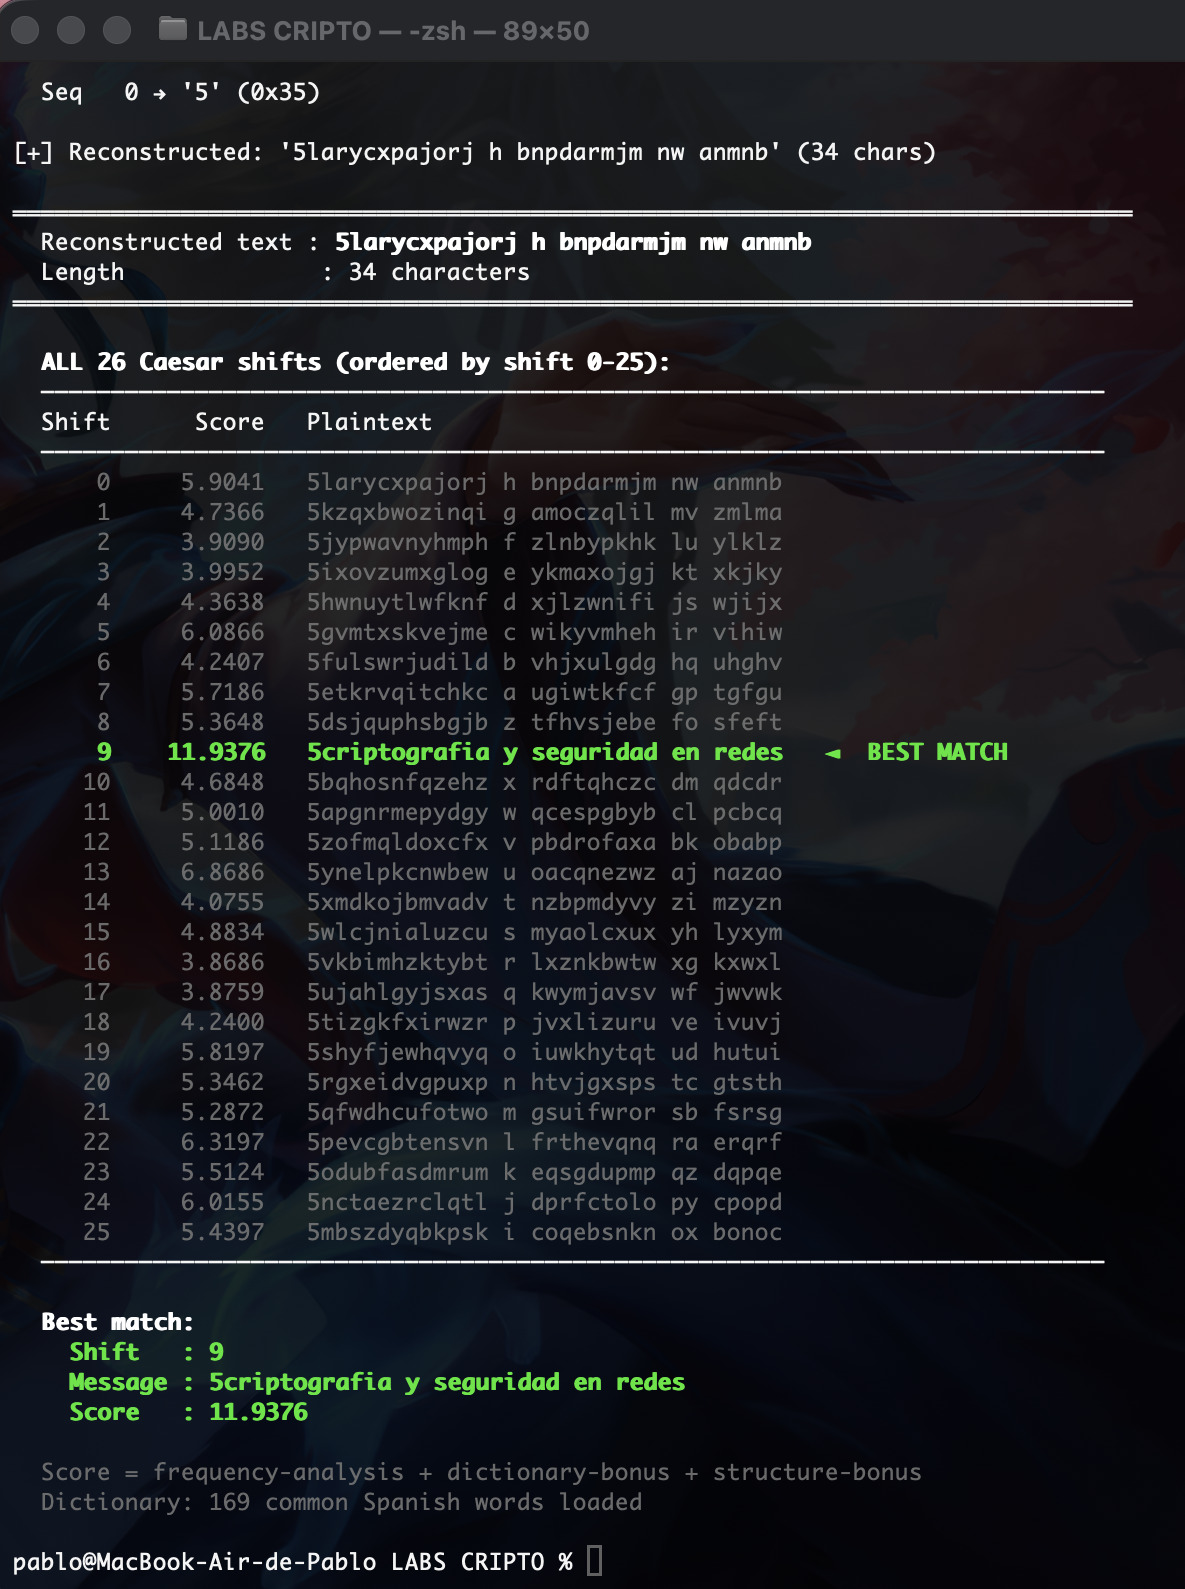
\includegraphics[width=\textwidth]{pcap2.jpg}
        \caption{Segunda parte de la ejecución}
        \label{fig:mitm2}
    \end{minipage}
    \caption{Ejecución de readv2.py mostrando las 26 combinaciones y la opción correcta en verde.}
    \label{fig:live-ejecucion}
\end{figure}

Se observa que el script logra identificar correctamente el mensaje en claro y el corrimiento utilizado, demostrando que \texttt{readv2.py} funciona correctamente con archivos PCAP y PCAPNG.

\subsubsection*{Captura en vivo}

Además de la lectura de archivos PCAP, \texttt{readv2.py} permite la captura en tiempo real de tráfico ICMP utilizando Scapy. En esta modalidad, el script escucha los paquetes entrantes y reconstruye el mensaje cifrado en el momento en que se transmite.

En la Figura~\ref{fig:live-ejecucion} se muestra la ejecución de \texttt{readv2.py} en modo captura en vivo, donde se transmitió el mensaje \textit{``HOLA AYUDANTES DE CRIPTO :\textgreater)''} cifrado con corrimiento 23. El script captura los paquetes ICMP, extrae los caracteres del payload y reconstruye el mensaje cifrado para luego probar las 26 combinaciones posibles del cifrado César.

\begin{figure}[H]
    \centering
    \begin{minipage}{0.48\textwidth}
        \centering
        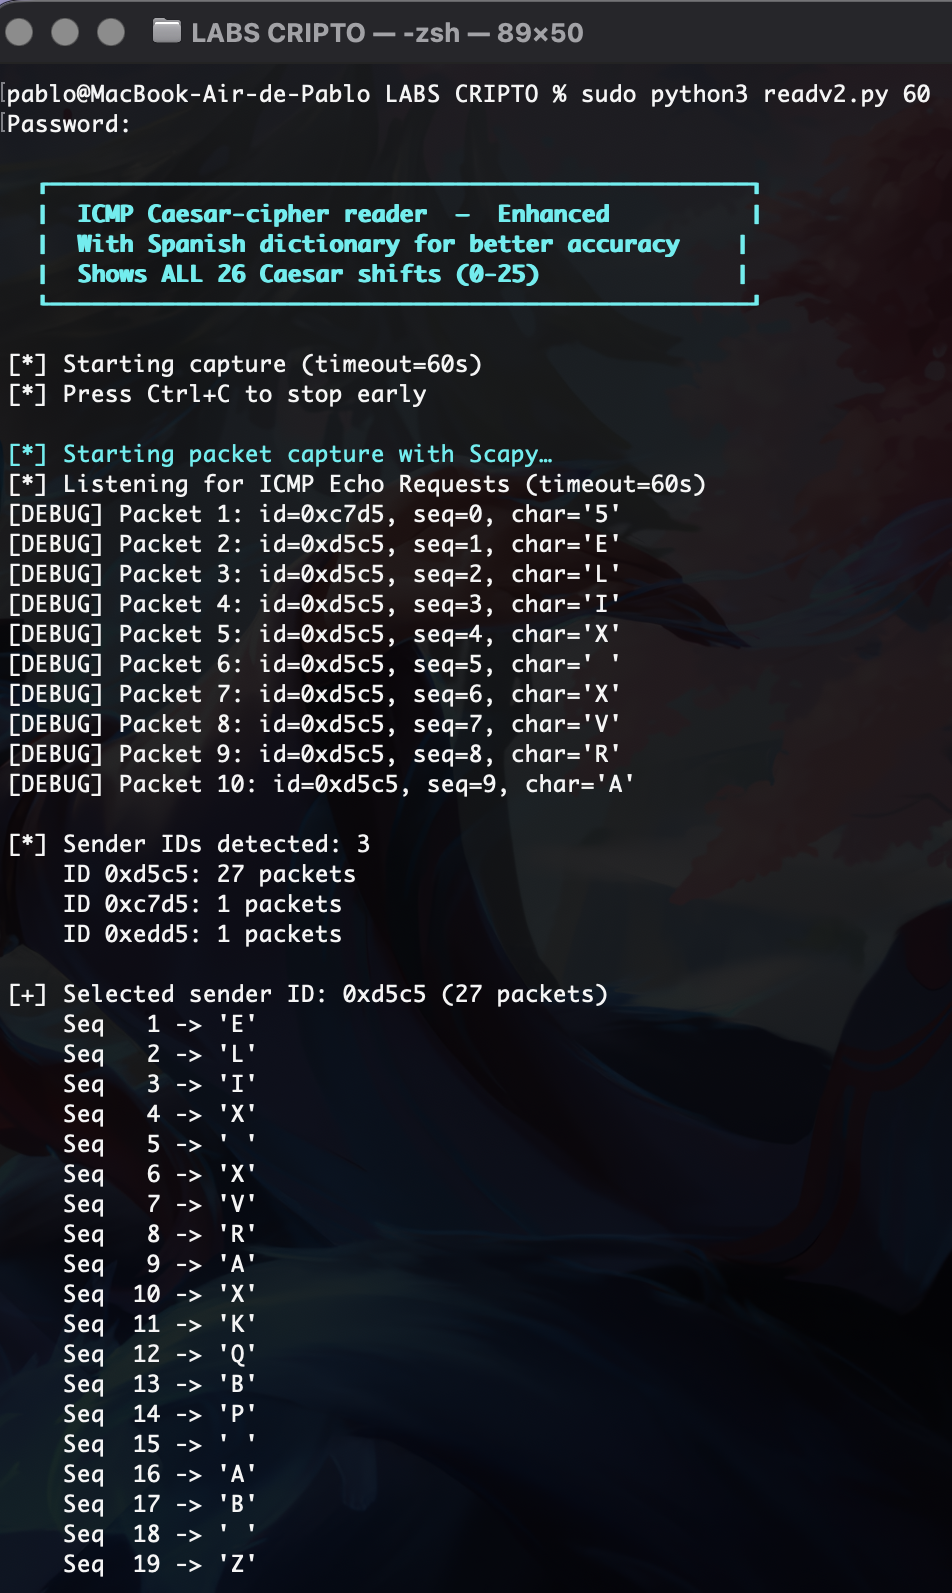
\includegraphics[width=\textwidth]{live1.png}
        \caption{Primera parte de la ejecución}
        \label{fig:live1}
    \end{minipage}
    \hfill
    \begin{minipage}{0.48\textwidth}
        \centering
        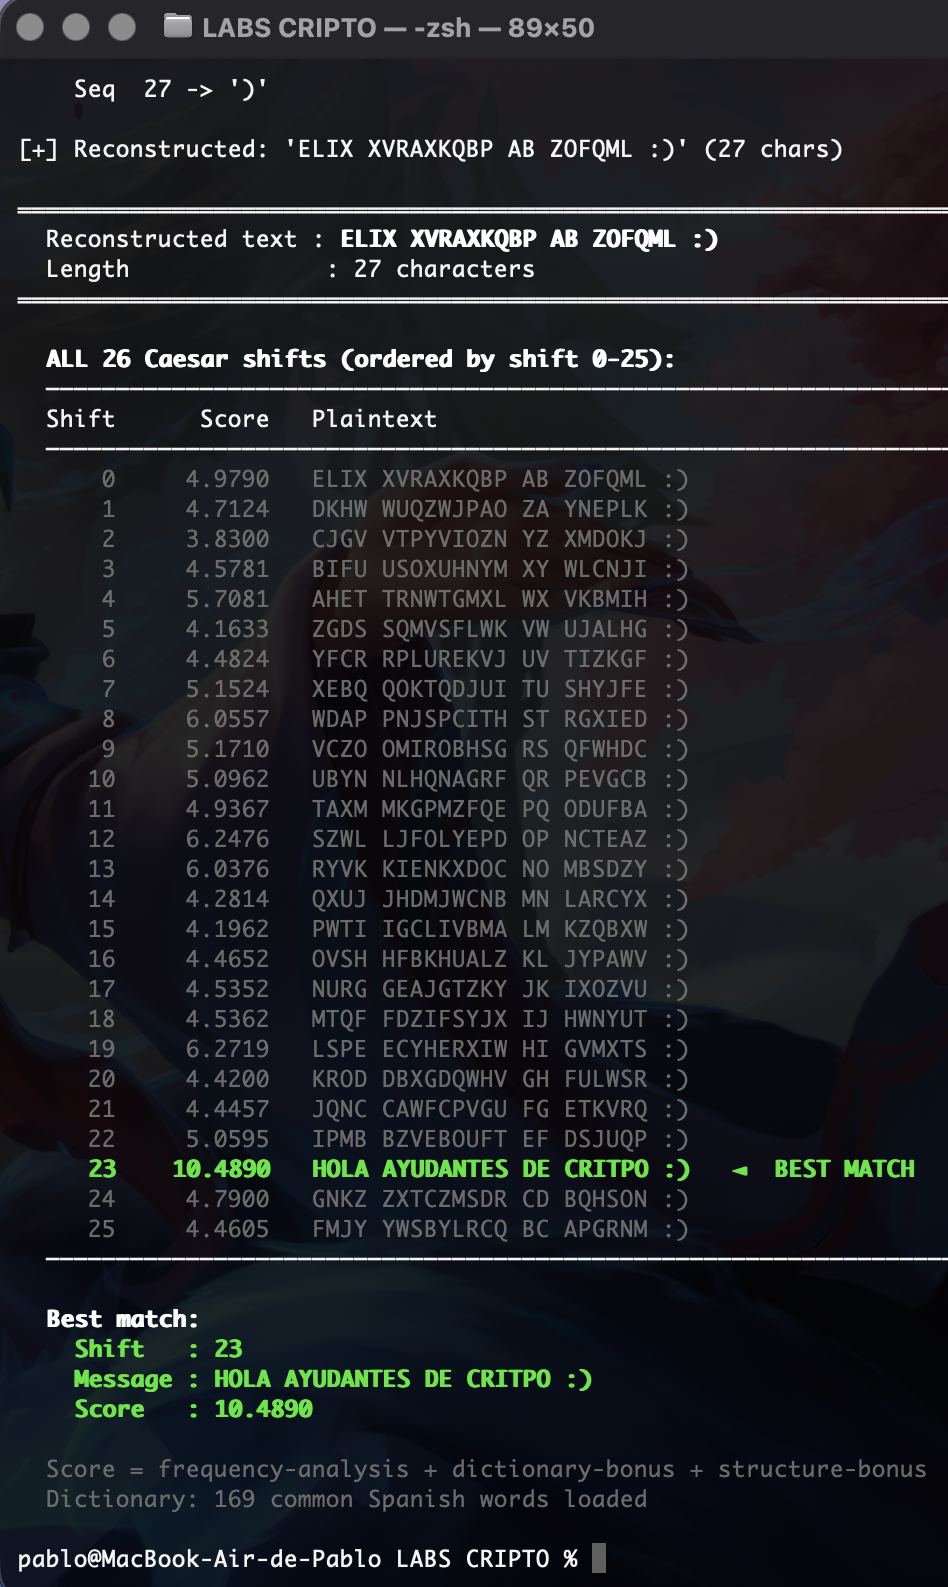
\includegraphics[width=\textwidth]{live2.png}
        \caption{Segunda parte de la ejecución}
        \label{fig:live2}
    \end{minipage}
    \caption{Ejecución de readv2.py en vivo mostrando las 26 combinaciones y la opción correcta en verde.}
    \label{fig:mitm-ejecucion}
\end{figure}

En la Figura~\ref{fig:live2} se observa el resultado final, donde el script identifica correctamente el corrimiento utilizado (\texttt{23}) y muestra el mensaje en claro \textit{``HOLA AYUDANTES DE CRIPTO :)''} destacado en verde. Esto demuestra que \texttt{readv2.py} funciona correctamente tanto en modo lectura de PCAP como en captura en vivo, logrando extraer y descifrar el mensaje oculto en el tráfico ICMP en tiempo real.

\subsubsection*{Ingreso de argumentos por terminal}

El script \texttt{readv2.py} soporta múltiples modos de operación mediante argumentos por línea de comandos:

\begin{itemize}
    \item \textbf{Modo PCAP} (\texttt{--pcap}): Analiza un archivo de captura previamente guardado en formato \texttt{.pcap} o \texttt{.pcapng}. El script extrae el mensaje cifrado de los paquetes ICMP almacenados y procede a descifrarlo. Es útil cuando se desea realizar un análisis diferido sin necesidad de generar tráfico en el momento.
    
    \item \textbf{Modo captura en vivo} (\texttt{timeout}): Escucha el tráfico ICMP en tiempo real durante un tiempo determinado (en segundos). Utiliza Scapy para capturar los paquetes entrantes, extraer los caracteres del payload y reconstruir el mensaje cifrado al momento de la transmisión. Es ideal para demostraciones en vivo o para capturar tráfico en el instante en que se genera.
    
    \item \textbf{Modo texto directo} (\texttt{--text}): Permite analizar un texto cifrado directamente, sin necesidad de capturar paquetes de red. El script aplica las 26 combinaciones del cifrado César y muestra los resultados. Es útil para pruebas rápidas o cuando ya se dispone del texto cifrado y solo se desea verificar el descifrado.
\end{itemize}

\begin{verbatim}
# Lectura de PCAP
sudo python3 readv2.py --pcap captura.pcap

# Captura en vivo (30 segundos)
sudo python3 readv2.py 30

# Análisis directo
sudo python3 readv2.py --text "larycxpajorj h bnpdarmjm nw anmnb"
\end{verbatim}

Esta flexibilidad permite al usuario analizar el tráfico ICMP tanto de forma diferida (con archivos PCAP) como en tiempo real, además de facilitar pruebas rápidas del algoritmo de descifrado sin necesidad de generar tráfico de red.

\subsubsection*{Algoritmo de scoring}

Para determinar cuál de las 26 combinaciones es la más probable, el script calcula un puntaje basado en:

\begin{enumerate}
    \item \textbf{Frecuencia de letras}: Compara la distribución de letras del texto con las frecuencias esperadas en español.
    \item \textbf{Palabras conocidas}: Busca palabras que coincidan con un diccionario de palabras comunes en español.
    \item \textbf{Estructura gramatical}: Evalúa la presencia de espacios, proporción de vocales y uso de letras comunes.
\end{enumerate}

La combinación con el puntaje más alto se considera la más probable y se destaca en verde.




% Please add the following required packages to your document preamble:
%\begin{table}[htbp]

\section*{Conclusiones y comentarios}

\subsection{Problemas y Soluciones}

Durante el desarrollo del laboratorio, se identificaron y resolvieron cuatro problemas principales al trabajar con DeepSeek y la implementación de los scripts.

\subsubsection*{Issue 1: Respuestas excesivamente complejas para problemas simples}

\textbf{Problema:} La IA utilizada a veces tomaba rutas largas y complicadas para resolver problemas simples. Inicialmente no estaba aplicando los 5 bytes en \texttt{0x00} en el payload ICMP, y comenzó a hacer modificaciones excesivas en el código que incluso lo rompían, generando errores de ejecución y paquetes mal formados.

\textbf{Solución:} Después de evaluar línea por línea el código generado, se identificó que la solución era simplemente agregar \texttt{b'\textbackslash x00' * 5} en la posición correcta del payload. Se le indicó directamente a la IA que solo agregara esos 5 bytes sin modificar el resto de la estructura, logrando así cumplir con el criterio de la pauta sin complicar innecesariamente el código.

\subsubsection*{Issue 2: Pérdida de contexto y modificaciones inconsistentes}

\textbf{Problema:} La IA utilizada presentaba poca memoria de contexto, cambiando constantemente partes del código que ya funcionaban correctamente. En varias ocasiones, modificaba el payload o la estructura de los paquetes sin motivo aparente, rompiendo funcionalidades que ya estaban implementadas y probadas.

\textbf{Solución:} Se mantuvo un registro constante del código original que funcionaba, y se le recordaba a la IA cuál era la versión estable cada vez que se desviaba. Se trabajó de forma iterativa, probando cada cambio antes de continuar, y se le pedía explícitamente a la IA que solo modificara lo necesario sin alterar el resto del código.

\subsubsection*{Issue 3: Dificultad para capturar paquetes ICMP en macOS}

\textbf{Problema:} Inicialmente no se podían capturar los paquetes ICMP generados por \texttt{pingv4.py} desde el script \texttt{readv2.py}. La IA no ayudó mucho en este problema, sugiriendo soluciones complejas que no funcionaban en macOS.

\textbf{Solución:} Después de consultar en un foro de Reddit, se llegó a la solución de instalar Scapy correctamente y configurarlo con los permisos adecuados en macOS. Una vez instalado, se trabajó con la IA para ajustar el script \texttt{readv2.py} para que utilizara Scapy de forma correcta, logrando capturar los paquetes ICMP en tiempo real.

\subsubsection*{Issue 4: Alineación incorrecta del payload y el padding}

\textbf{Problema:} Inicialmente, el script insertaba el carácter inyectado justo después del patrón \texttt{0x10-0x37}, lo que provocaba que el padding comenzara con el carácter en lugar de la secuencia \texttt{00 01 02 03...} que espera un analista de tráfico. Esto podría levantar sospechas ante un sistema DPI, ya que el padding del ping real de macOS es una secuencia incremental predecible.

\textbf{Solución:} Se modificó el script para que el carácter inyectado reemplace el primer byte del padding en lugar de interrumpir la secuencia del patrón. De esta forma, el padding mantiene su estructura normal (\texttt{61 01 02 03 04...}) y el patrón \texttt{0x10-0x37} permanece completamente intacto, haciendo que el tráfico sea prácticamente indistinguible del ping real.

\subsection{Comentarios Finales}

El trabajo con DeepSeek resultó productivo, aunque requirió varias iteraciones para ajustar los scripts a los requisitos específicos del laboratorio y a las particularidades del sistema operativo macOS. La principal lección aprendida fue la importancia de conocer en detalle el comportamiento del tráfico real que se desea replicar para lograr un verdadero stealth.

Los principales logros del laboratorio fueron:
\begin{itemize}
    \item Implementación exitosa del cifrado César con argumentos por terminal.
    \item Generación de tráfico ICMP indistinguible del ping real de macOS, replicando todos los campos relevantes (timestamp, checksum, identifier, sequence, payload).
    \item Desarrollo de un sistema MitM capaz de capturar, extraer y descifrar el mensaje oculto.
    \item Identificación y resolución de 4 issues críticos relacionados con macOS y las herramientas utilizadas.
\end{itemize}

Se destaca la importancia de la validación constante del tráfico generado mediante herramientas como Wireshark, ya que pequeños detalles en el payload pueden hacer que el tráfico sea detectable por sistemas DPI. La experiencia con DeepSeek demostró que, si bien es una herramienta poderosa, requiere supervisión y corrección constante para evitar desviaciones del objetivo original.

\section{Anexos}

El código fuente completo de los scripts desarrollados para este laboratorio se encuentra disponible en el siguiente repositorio de GitHub:

\begin{itemize}
    \item \textbf{Repositorio:} \url{https://github.com/Pablomvnzr/LAB1Cripto}
    \item \textbf{Descripción:} Scripts en Python para cifrado César, filtración de datos por ICMP y captura/descifrado de tráfico.
    \item \textbf{Última actualización:} 4 de septiembre de 2026
\end{itemize}

Los archivos incluidos son:
\begin{itemize}
    \item \texttt{cesar.py}: Implementación del cifrado César.
    \item \texttt{pingv4.py}: Script para inyectar datos en tráfico ICMP (modo stealth).
    \item \texttt{readv2.py}: Script para capturar y descifrar el mensaje oculto.
    \item \texttt{testpcap.pcapng}: Archivo de captura de prueba.
    \item \texttt{README.md}: Documentación del proyecto.
\end{itemize}

\end{document}
